\documentclass[10pt,a4paper]{article}
\usepackage[UTF8]{ctex}
\usepackage{tikz}  
\usepackage{amsmath}
\usepackage{amsfonts}
\usepackage{amssymb}
\usepackage{float}
%\usepackage{clrscode}
\usepackage[]{algorithm2e}
\usepackage{graphicx}
% Set the margin of document.
\usepackage[top=10mm, bottom=12.5mm, left=12.5mm, right=12.5mm]{geometry}
\usepackage{longtable}
\usepackage{float}
\usepackage{listings}
\lstset{
  basicstyle=\small,
  numbers=left,
  keywordstyle=\color{blue},
  numberstyle={\tiny\color{lightgray}},
  stepnumber=1, %行号会逐行往上递增
  numbersep=5pt,
  commentstyle=\small\color{red},
  backgroundcolor=\color[rgb]{0.95,1.0,1.0},
  showspaces=false,
  showtabs=false,
  frame=shadowbox, framexleftmargin=5mm, rulesepcolor=\color{red!20!green!20!blue!20!},
% frame=single,
%  TABframe=single,
  tabsize=4,
  breaklines=tr,
  extendedchars=false %这一条命令可以解决代码跨页时,章节标题,页眉等汉字不显示的问题
}
\renewcommand\figurename{图}
\renewcommand\tablename{表}
\title{实验数据的拟合}
\author{袁略真\\3130103964\\生物信息学\\浙江大学}
\begin{document}
\maketitle

\section{使用线性回归进行数据拟合}
物理量$x,y$遵循某种未知的函数关系$y=f(x)$. 为了确定这个目标函数关系,通常需要实验测量,获得n组数据. 对这些数据应用恰当的统计模型,可以描述尽可能真实的规律($y=y(x)$),也就是接近真实的函数关系($y(x)\approx f(x)$).

本节课使用的统计模型是线性回归模型$y(x)=A_0+A_1x$, 选定的拟合标准为最小二乘法,也就是拟合曲线与测量数据有偏差平方和最小. 对于多选线性拟合的情形,模型做适当拓展即可.

\subsection{非线性关系的线性拟合}
当物理量$x,y$遵循非线性函数关系时,如果仍要使用线性回归模型的方法拟合非线性模型(如$y=Ae^{Bx}$),需要将数据进行适当转换($Y'=lny,x'=x. Y' = lnA + Bx'$).

\section{程序流程}
\begin{enumerate}
\item Generate standard deviation for average~N
\item Transform the data
\begin{lstlisting}[language=c++]
ind = 0;
if(y(N) = a e^{bN})
	Y'=lny;N'= N;ind = 1;//lnY = lna + bx
else if(y(N) = a N^b)
	Y'=lny;N' = lnN;ind = 2//lnY = lna + blnN
\end{lstlisting}


\item Several average calculation: $\bar{x}, \bar{y}, \bar{xy}, \bar{x^2}, n=length(Y')$;
\item Linear correlation coefficient:
\begin{lstlisting}[language=c++]
ab=0;a2=0;b2=0;
for i=1:n:
	a = (x_i-\bar{x});
	b = (y_i-\bar{y});
	ab + = a*b;
	a2 += a*a;b2 += b*b;
end for
r = a*b/(a2 * b2)^0.5
\end{lstlisting}


\item Linear fitting:
\begin{lstlisting}[language=c++]
A1 = (\bar{xy} - \bar{x} * \bar{y})/(\bar{x^2} - \bar{x}^2);
A0 = \bar{y} - A1 * \bar{x};

tmp = 0;
for i = 1:n:
	tmp += (yi - A0 - A1 * xi)^2;
sigma = (1/(n-2) * tmp)^0.5;//standard deviation
sigmaA0 = sigma * (\bar{x^2}/(n*\bar{x^2} - \bar{x}^2 ) )^0.5;
sigmaA1 = sigma * (1/(n*\bar{x^2} - \bar{x}^2 ) )^0.5
\end{lstlisting}


\item Transform back
\begin{lstlisting}[language=c++]
a = e^A0;b=A1;

if(ind == 1 or ind == 2)
	y'pred = e(A0 + A1*N');//predicted y
	ypred = e^{y'pred};
	cout<<N<<y<<ypred;
\end{lstlisting}

\end{enumerate}

\section{拟合结果}
\subsection{拟合参数和标准偏差}

\begin{table}[H]
\begin{minipage}[b]{0.5\linewidth}\centering
\begin{tabular}{|c|c|}
\hline
Final Model&$y(N) = 0.0042296e^{-0.0281388N}$\\
\hline
cc$^*$&-0.909336\\
$A_0$&-5.46565\\
$A_1$&-0.0281388\\
$a$&0.0042296\\
$b$&-0.0281388\\
$\sigma$&0.189625\\
$\sigma_{A_0}$&0.0270225\\
$\sigma_{A_1}$&0.000922264\\
\hline
\end{tabular}
\caption{$Y(N)=a e^{bx}$. $^*$: correlation coefficient}
\end{minipage}
\hspace{0.5cm}
\begin{minipage}[b]{0.5\linewidth}\centering
\begin{tabular}{|c|c|}
\hline
Final Model&$y(N) = 0.00911777N^{-0.499482}$\\
\hline
cc$^*$&-0.998902\\
$A_0$&-4.69753\\
$A_1$&-0.499482\\
$a$&0.0042296\\
$b$&-0.0281388\\
$\sigma$&0.0210493\\
$\sigma_{A_0}$&0.00300457\\
$\sigma_{A_1}$&0.000970073\\
\hline
\end{tabular}
\caption{$Y(N)=a e^{bx}$. $^*$: correlation coefficient}
\end{minipage}
\end{table}
\subsection{图形结果}
\begin{figure}[H]
\begin{minipage}[b]{0.5\linewidth}
\centering
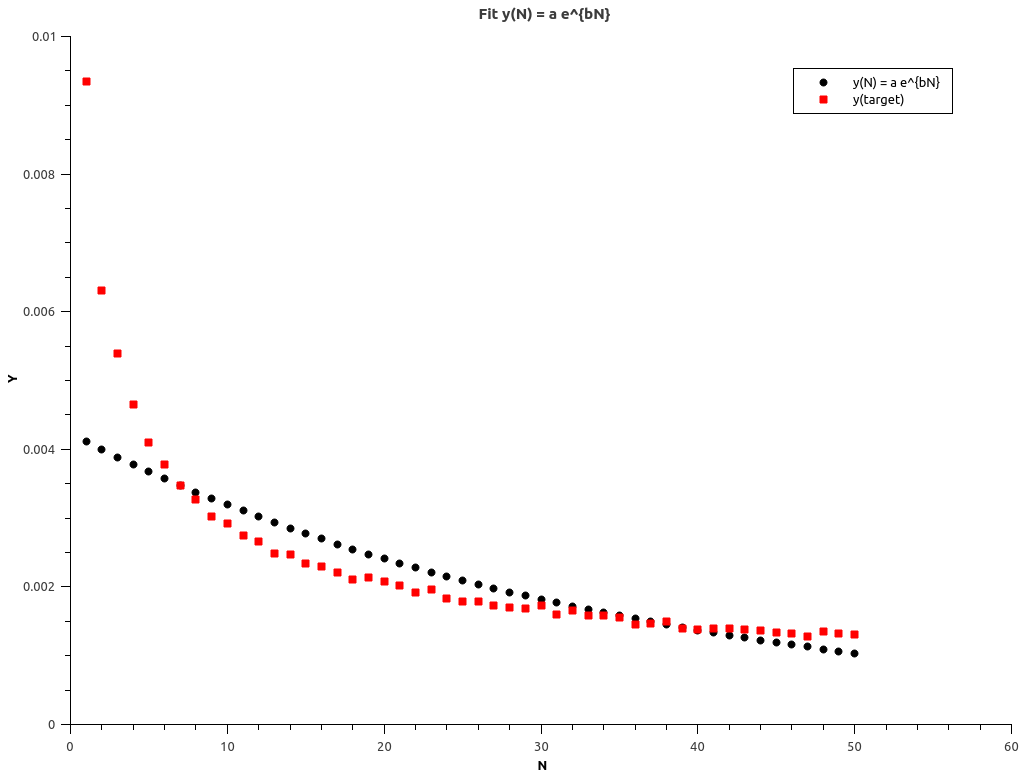
\includegraphics[width=\textwidth]{../result/Graph1.png}
\caption{\textbf{使用$Y(N)=a e^{bx}$对$\sigma_{\bar{x}}\sim N$做线性拟合.} 数据先调整为$y'=lny,x'=x$(线性相关系数-0.909336),然后使用线性回归模型$y(x)=A_0+A_1x$进行拟合. 拟合直线标准偏差0.189625.}
\label{fig:1}
\end{minipage}
\hspace{0.5cm}
\begin{minipage}[b]{0.5\linewidth}
\centering
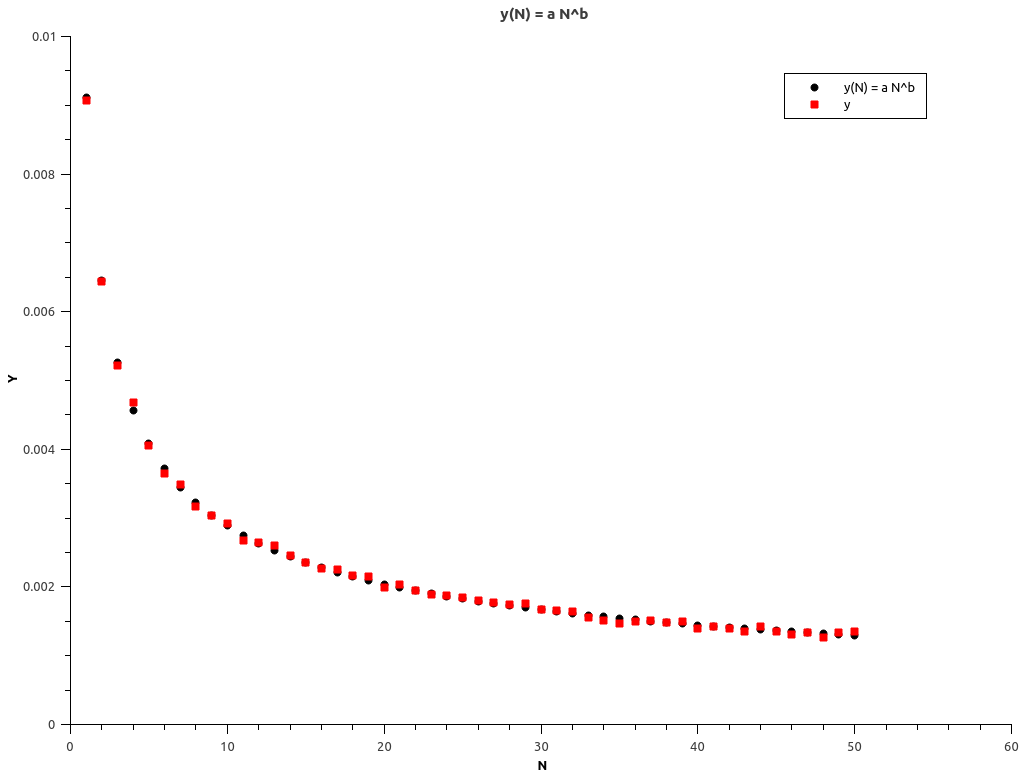
\includegraphics[width=\textwidth]{../result/Graph2.png}
\caption{\textbf{使用$Y(N)=a N^{b}$对$\sigma_{\bar{x}}\sim N$做线性拟合.} 数据先调整为$y'=lny,x'=lnx$(线性相关系数-0.998902),然后使用线性回归模型$y(x)=A_0+A_1x$进行拟合. 拟合直线标准偏差0.0210493.}
\label{fig:2}
\end{minipage}
\end{figure}
\end{document}